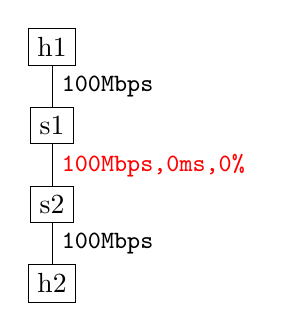
\begin{tikzpicture}
    \tikzstyle{host}=[draw]
    \tikzstyle{switch}=[draw]
    \tikzstyle{connection}=[]
    \tikzstyle{constr}=[right,font=\ttfamily\small]
    \node [host] (h1) at (0,4) {h1};
    \node [switch] (s1) at (0,3) {s1};
    \node [switch] (s2) at (0,2) {s2};
    \node [host] (h2) at (0,1) {h2};
    \draw (h1) edge node [constr] {100Mbps} (s1);
    \draw (s1) edge node [constr] {\color{red} 100Mbps,0ms,0\%} (s2);
    \draw (s2) edge node [constr] {100Mbps} (h2);
\end{tikzpicture}